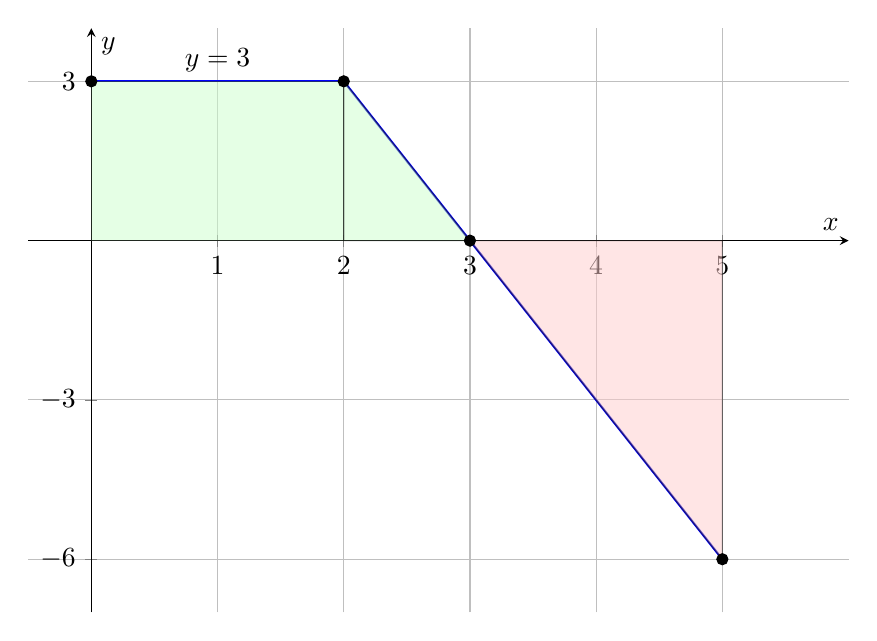
\begin{tikzpicture}
\begin{axis}[
    axis lines=center,
    xlabel=$x$, ylabel=$y$,
    xmin=-0.5, xmax=6,
    ymin=-7, ymax=4,
    width=12cm, height=9cm,
    xtick={0,1,2,3,4,5},
    ytick={-6,-3,0,3},
    grid=major
]

% Define the piecewise function
% Rectangle: y = 3 on [0, 2]
\addplot[blue, thick, domain=0:2] {3};

% Diagonal line from (2,3) to (5,-6)
% Slope = (-6-3)/(5-2) = -9/3 = -3
% y - 3 = -3(x - 2) => y = -3x + 9
\addplot[blue, thick, domain=2:5] {-3*x + 9};

% Fill rectangle area [0,2]
\addplot[fill=green!20, opacity=0.5] coordinates {(0,0) (2,0) (2,3) (0,3) (0,0)};

% Fill triangle area [2,3] (above x-axis)
\addplot[fill=green!20, opacity=0.5] coordinates {(2,3) (3,0) (2,0) (2,3)};

% Fill triangle area [3,5] (below x-axis)
\addplot[fill=red!20, opacity=0.5] coordinates {(3,0) (5,0) (5,-6) (3,0)};

% Mark key points
\addplot[only marks, mark=*, mark size=2pt] coordinates {(0,3) (2,3) (3,0) (5,-6)};

% Labels
\node[above] at (axis cs:1,3) {$y=3$};

\end{axis}
\end{tikzpicture}
